\chapter{Event Reconstruction and Selection}\label{ch:event_selection}

Events are recorded and reconstructed in the CMS detector, then further selection criteria are imposed in order to determine analysis-level physics objects. General event reconstruction will be discussed, followed by the specific diphoton event selection used in this analysis.


\section{Event Reconstruction}\label{sec:event_reco}

After events are recorded by the CMS detector, they are reconstructed through a variety of algorithms into their constituent components. All electrically charged particles produce signals in the pixel and strip tracking system. Muons are detected within the muon system before, generally, leaving the detector. Electrons and photons deposit most of their energies in the ECAL, while charged and neutral hadrons mostly deposit in the HCAL. The electrical signals produced by each subdetector are read out and converted into physics object candidates. Each subdetector can individually generate different particle candidates; however, CMS uses particle-flow (PF) global event reconstruction~\cite{CMS-PRF-14-001} to identify and reconstruct individual particles (namely, electrons, muons, photons, charged hadrons, and neutral hadrons) using information from all subdetectors. Jets, missing transverse energy, and other composite objects are built using the PF algorithm.

\subsection{Tracks and Vertices}\label{sec:track_vertex}

The trajectories of charged particles form tracks as they propagate as helices between the tracker layers. Tracks are fundamental for event reconstruction, contributing towards the subsequent reconstruction of other physics objects in the event. CMS uses the Combinatorial Track Finder (CTF) algorithm, which is based on a Kalman filter, for track reconstruction, as described in Ref.~\cite{Chatrchyan:2014fea}. The CTF fits tracker hits, while taking into account the uncertainty of the hit positions and the effects of multiple Coulomb scattering and energy loss. The fit returns track information, including charge, initial momentum, and its impact parameter with respect to the primary vertex.

Primary vertices are those compatible with the hard scattering from the pp interactions along the beam line. Secondary vertices in the event can result from particle decays after the hard interaction. The primary vertex is reconstructed by selecting and clustering tracks compatible with the LHC beam spot, which is the 3D luminous region where the LHC beams collide. The track clustering is done using a deterministic annealing algorithm, and the position of each vertex is fit for using its associated tracks, as described in Ref.~\cite{Chatrchyan:2014fea}. Due to pileup, multiple primary vertices can be reconstructed in an event. However, the main primary vertex is chosen to be the reconstructed vertex with the largest value of summed charged-particle track $\pt^2$, with additional constraints described in Section~9.4.1 of Ref.~\cite{Contardo:2020886}. This selected vertex is simply referred to as the primary vertex. The position resolution for primary vertices is between 10-12~$\mu$m for each of its three spatial coordinates~\cite{Chatrchyan:2014fea}.


\subsection{Photons and Electrons}

Photon candidates are reconstructed from energy deposits in the ECAL. Before entering the ECAL, a photon may convert in the tracker into an electron-positron pair, whose paths bend under the influence of the magnetic field, causing their energy deposits to be extended along the $\phi$ direction. Individual energy deposits are grouped into superclusters to allow maximal recovery, using different procedures in the EB and EE regions. ECAL crystals are aligned in an $(\eta, \phi)$ grid in the EB and an $(x, y)$ grid in either EE. First, clusters are built starting with a seed crystal, which is located by selecting the crystal with the highest $E_{\mathrm{T}}$ above a certain threshold among its neighboring crystals. Next, in the EB region, a $5{\times}1$ bar of crystals centered on a seed is formed along the $\eta$ direction. Connected bars within $\pm17$ crystals along $\phi$ from the seed crystal are added if their total energy is above some threshold, forming a cluster. Other clusters, built in this way, having seeds aligned in $\eta$ with this cluster's seed are added, based on a further threshold requirement, to form superclusters. In the EE regions, a cluster of a $5{\times}5$ array of crystals centered on a seed is first built. The crystals surrounding the $5{\times}5$ boundary are allowed to seed new $5{\times}5$ clusters using crystals not included in any cluster yet. The clusters are allowed to partially overlap, and a supercluster is formed from the connected clusters. In either the EB or an EE, the superclusters formed for unconverted photons are typically $5{\times}5$ matrices. Further details are described in Ref.~\cite{CMS:EGM-14-001}.

The raw energy for photons is obtained by summing the energy deposits in the supercluster, corrected for detector effects, as described in Section~\ref{sec:ECAL}. Energy deposited in an ECAL preshower detector is added to the photon energy measurement from the adjacent EE. This \correction{raw energy needs to be corrected,} mainly to account for photon shower loss and contamination from pileup. The shower may be lost between gaps in the crystals or through gaps in the ECAL modules, resulting in parts of the shower not being clustered into the supercluster. Data-driven scale factors for the photon energy scale and resolution are extracted from $Z \to e^+e^-$ decays, with electrons reconstructed as photons, using an energy regression based on a boosted decision tree (BDT)~\cite{CMS:EGM-14-001}. Because of the limited dynamic range of the ECAL readout electronics, they saturate when the energy deposited in a single crystal is greater than an average value of about 1.7 (2.8)\TeV in the EB (EEs), with a spread of about 10 (25)\% among different channels. Energy corrections to account for this are derived using a simulated sample of photon candidates with energies spanning a large range. The photon energy scale and resolution are corrected by comparing the difference between data and simulation from $Z \to e^+e^-$ events, calibrated at the $Z$ boson peak. The difference in energy scale is used to correct the data. The energy resolution in simulation needs additional Gaussian smearing to match that of data, which is considered as a correction. In the EB, photons in the range of tens of {\GeVns} have an energy resolution of about 1\%, while photons above this range have a resolution of about 1.3\% up to $|\eta| = 1$, rising to about 2.5\% at $|\eta| = 1.4$. In each EE, the energy resolution for photons in the range of tens of {\GeVns} is about 2.5\%, while photons above this range have a resolution between 3 and 4\%~\cite{CMS:EGM-14-001}.

Electrons are reconstructed by matching a track to an ECAL supercluster, determined using the same method as for photons. The electron track reconstruction uses a Gaussian sum filter (GSF) to fit the tracker hits. The emitted bremsstrahlung photons, which can carry away a significant fraction of the initial electron energy, can convert into electron-positron pairs, yielding secondary tracks. This is taken into account by the GSF. The details are described in Ref.~\cite{Khachatryan:2015hwa}.


\subsection{Muons and Tau Leptons}

Muon reconstruction uses information from both the muon system and inner tracker. Muon tracks are first reconstructed in the muon system to form track segments generated by requiring a certain number of hits in the layers within a single DT or CSC chamber. These segments are then fit, with information from the RPCs included, to form standalone muons. These standalone candidates are then matched to tracks from the inner tracking system by projecting the standalone muon trajectories to the outer tracker surface and using a method similar to the CTF algorithm (see Ref.~\cite{Sirunyan:2018fpa} for details). Muon performance was discussed in Chapter~\ref{ch:experiment}.

The $\tau$ lepton signature is more complex than for electrons or muons. They are the heaviest of the charged leptons, with a short lifetime, and will typically decay before reaching the active material of the detector. About 2/3 of the time, $\tau$ leptons decay hadronically and can be reconstructed indirectly through their PF candidate decay products. The performance of $\tau$ lepton reconstruction and identification is presented in Refs.~\cite{Chatrchyan:2012zz,Sirunyan:2018pgf}.

\subsection{Jets and Missing Transverse Energy}\label{sec:jets}

A typical proton-proton collision will produce quarks or gluons either through the hard interaction directly or through QCD radiation from the initial or final state partons. Due to QCD confinement, colored partons are not freely observed. Instead, they transform into a collection of color-neutral hadrons, observed as a cluster of particles called jets. Because the number of color states for gluons is larger than for quarks, gluon-initiated jets, in general, have higher particle multiplicity, a softer fragmentation function, and are less collimated than quark-initiated jets~\cite{CMS:2013kfa,Aad:2014gea}. So, quark jets tend to have lower multiplicity, harder constituents, and are narrower. In addition, quarks have electrical charge, while gluons do not. Jets can be further classified according to their quark flavor. Heavy-flavor jets originate from $b$ or $c$ quarks, while light-flavor jets are those originating from $u$, $d$, or $s$ quarks. In some cases, jet identification techniques are able to discriminate between these different types of jets~\cite{Asquith:2018igt,Sirunyan:2017ezt}. Top quarks decay before they hadronize and are identified through their decay products (see, e.g., Ref.~\cite{Sirunyan:2017huu}).

Jets are built from PF candidates, primarily detected as charged hadrons (e.g., $\pi^{\pm}$, $K^{\pm}$, and protons), neutral hadrons (e.g, $K^0_{\mathrm{L}}$ and neutrons), or nonisolated photons (e.g., from $\pi^0$ decays). The energy deposits are calibrated to account for the nonlinear response of the calorimeters, and reconstructed tracks are compared to the clusters. The energy deposits are clustered into jets using the infrared and collinear safe anti-$k_{\mathrm{T}}$ algorithm~\cite{Cacciari:2008gp,Cacciari:2011ma}, with a distance parameter of $R = 0.4$. Infrared (collinear) safety means the jet algorithm remains invariant under soft emission (co-moving / collinear momentum splitting) of the clustered particles. Heavy-flavor jets will typically produce a secondary vertex. For example, a $B$ meson such as a $B^{+}$ will travel an average distance of approximately 500~$\mu$m before decaying. This is well within the vertex resolution of the tracking system. Jets originating from $b$ quarks are identified with the combined secondary vertex (CSVv2) $b$ tagging algorithm~\cite{Sirunyan:2017ezt}. Since the lifetime of a $c$ quark is shorter than that of a $b$ quark, a similar, but modified, procedure is used for $c$ jet identification, discussed in Ref.~\cite{Sirunyan:2017ezt}.

Neutrinos interact only through the weak interaction and escape through the detector. This is also true for any (stable) electrically neutral, colorless particle. Nonetheless, their presence can be inferred through a momentum imbalance in the collision using conservation of momentum, given that the initial transverse momentum of the colliding system is negligible. In the transverse plane, this would show up as missing $E_\mathrm{T}$, referred to as MET, equal to $\left| -\sum{\vec{\pt}}\right|$. Along the longitudinal axis, the missing $E_\mathrm{z}$ is not useful since the initial longitudinal momenta of the colliding partons within the protons are unknown.


\section{Event Selection}

The signature in this analysis consists of two high-energy, prompt photons. Events containing this signature are reconstructed and required to pass a trigger selection. These photons form diphoton candidates, which are required to pass a preselection and further identification criteria, imposed to obtain high event purity with high search sensitivity.

\subsection{Trigger Selection}\label{sec:trigger}

Events are selected which pass the CMS HLT trigger with path name \texttt{HLT\_DoublePhoton60}. These events contain at least two photon candidates, each with $\pt>60\GeV$, across the range $|\eta| < 3.0$. The primary selection at this level requires each photon candidate to have $\hoe < 0.15$. The longitudinal shower shape variable $\hoe$ is defined as the ratio of the hadronic to electromagnetic energy fraction of the photon candidate. The electromagnetic energy fraction is defined as the corrected supercluster energy. At this trigger level, the hadronic energy fraction is defined as the total HCAL energy within a cone of $\Delta R < 0.15$ from the supercluster position, as used in the variable referred to as $\text{Hadronic/E}$ in Section~\ref{sec:fake_background}. Later, at the analysis level, this fraction will mean the amount of HCAL energy in the tower directly behind the photon seed crystal. This trigger is seeded by the logical OR of a suite of \texttt{SingleEG}, \texttt{DoubleEG}, \texttt{SingleJet}, and \texttt{SingleTau} CMS L1 seeds, with varying thresholds. These thresholds are primarily sensitive to one or two large electromagnetic energy deposits, a large hadronic energy deposit, or a signature in the muon and calorimeter systems consistent with the presence of a single $\tau$ lepton decay, respectively.

The trigger efficiency measured relative to the \texttt{HLT\_DoublePhoton40} trigger, which requires the two photon candidates to each have $\pt>40\GeV$, is shown in Fig.~\ref{fig:relative_trigger_efficiency}. The photons are ordered by \pt in each event, with the leading photon having the highest \pt and the subleading photon having the second highest. The efficiency shown here is measured as a function of the subleading photon \pt. This selection is fully efficient above photon $\pt > 75\GeV$.

\begin{figure}[!htbp]
	\centering
	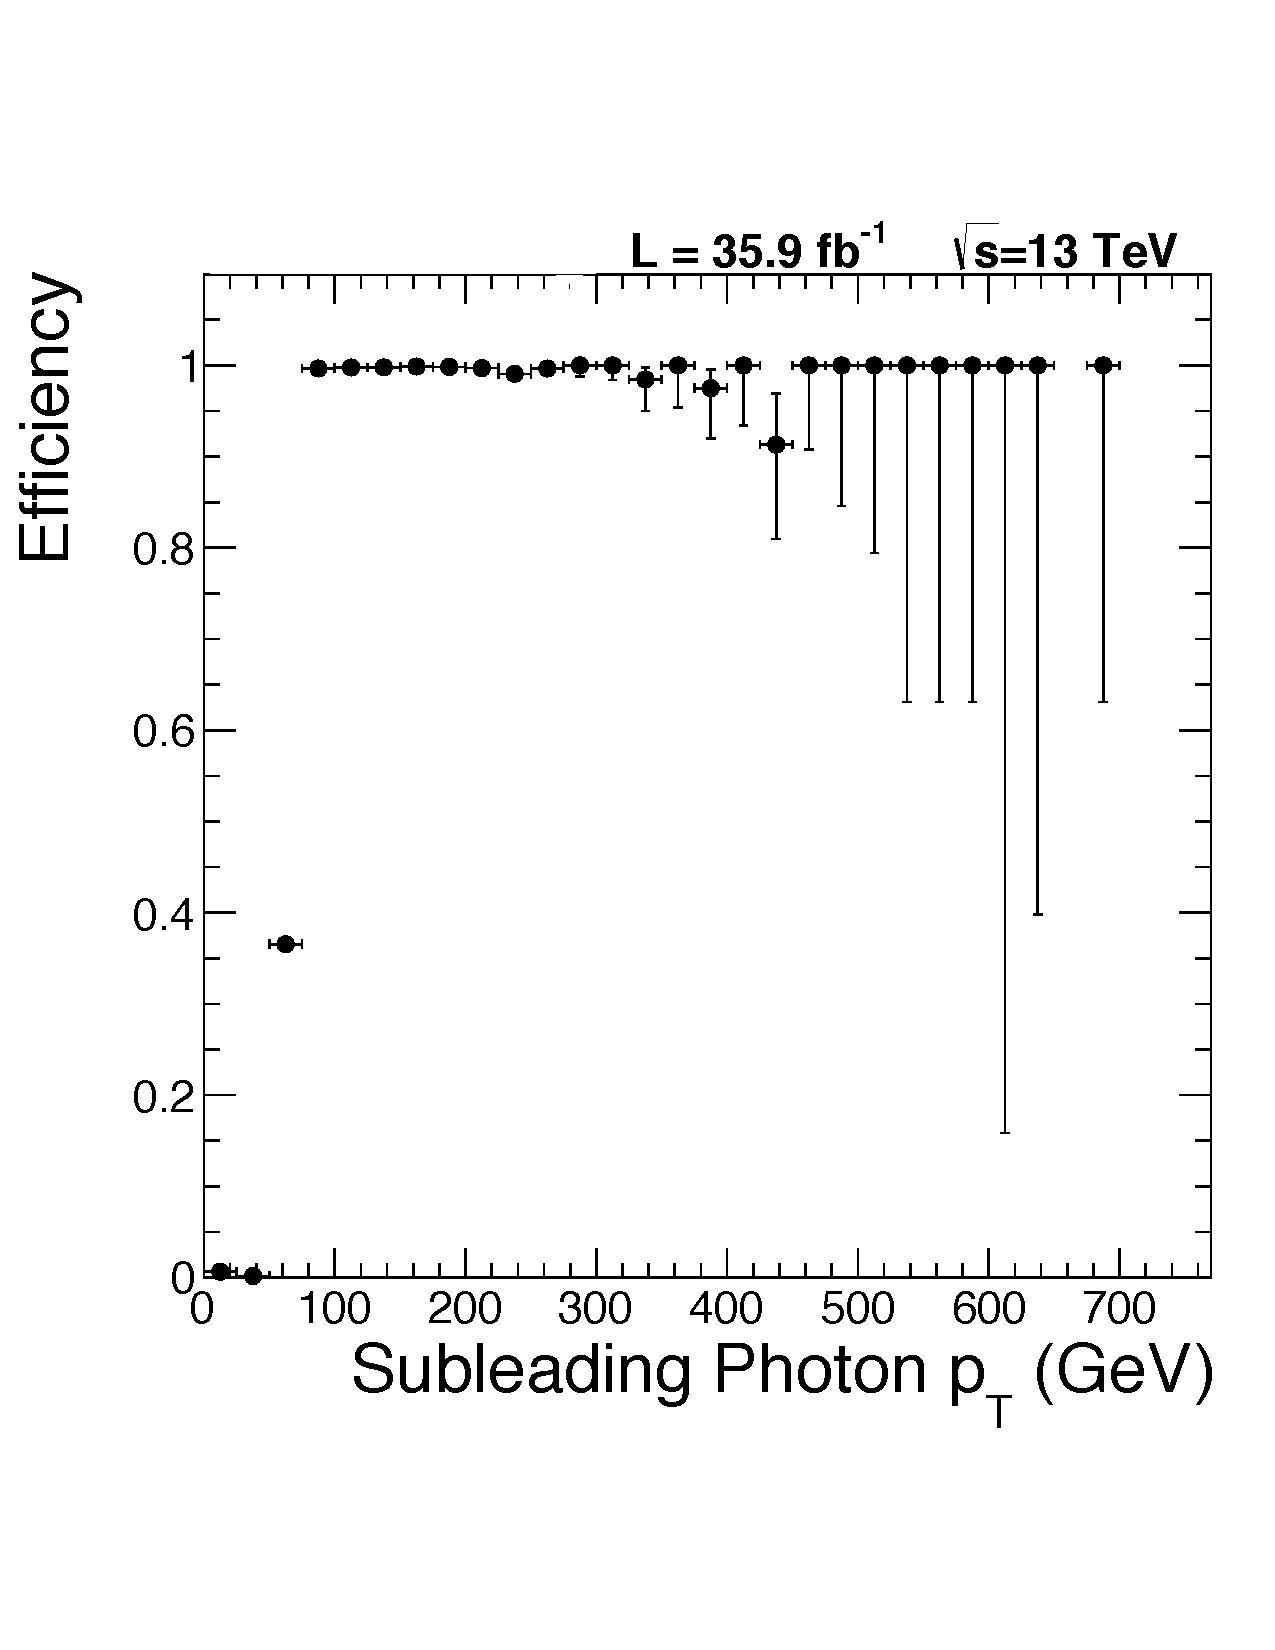
\includegraphics[angle=0,width=0.55\textwidth]{figures/eff2016.pdf}
	\caption{The relative efficiency of the \texttt{HLT\_DoublePhoton60} trigger (measured with reference to the \texttt{HLT\_DoublePhoton40} trigger) as a function of the \pt of the subleading photon.}
	\label{fig:relative_trigger_efficiency}
\end{figure}

The absolute trigger efficiency of \texttt{HLT\_DoublePhoton60} was measured using a simulated sample of diphoton events, similar to those described in Chapter~\ref{ch:signal}. In this simulated sample, the diphoton invariant mass \mgg is known and can be compared before and after imposing the trigger selection. Fig.~\ref{fig:absolute_trigger_efficiency} shows the trigger efficiency as a function of \mgg, which is fully efficient for events with $\mgg > 500\GeV$. The two plots shown correspond to the different analysis event categories, which will be explained in the following section.

\begin{figure}[!htbp]
	\centering
  	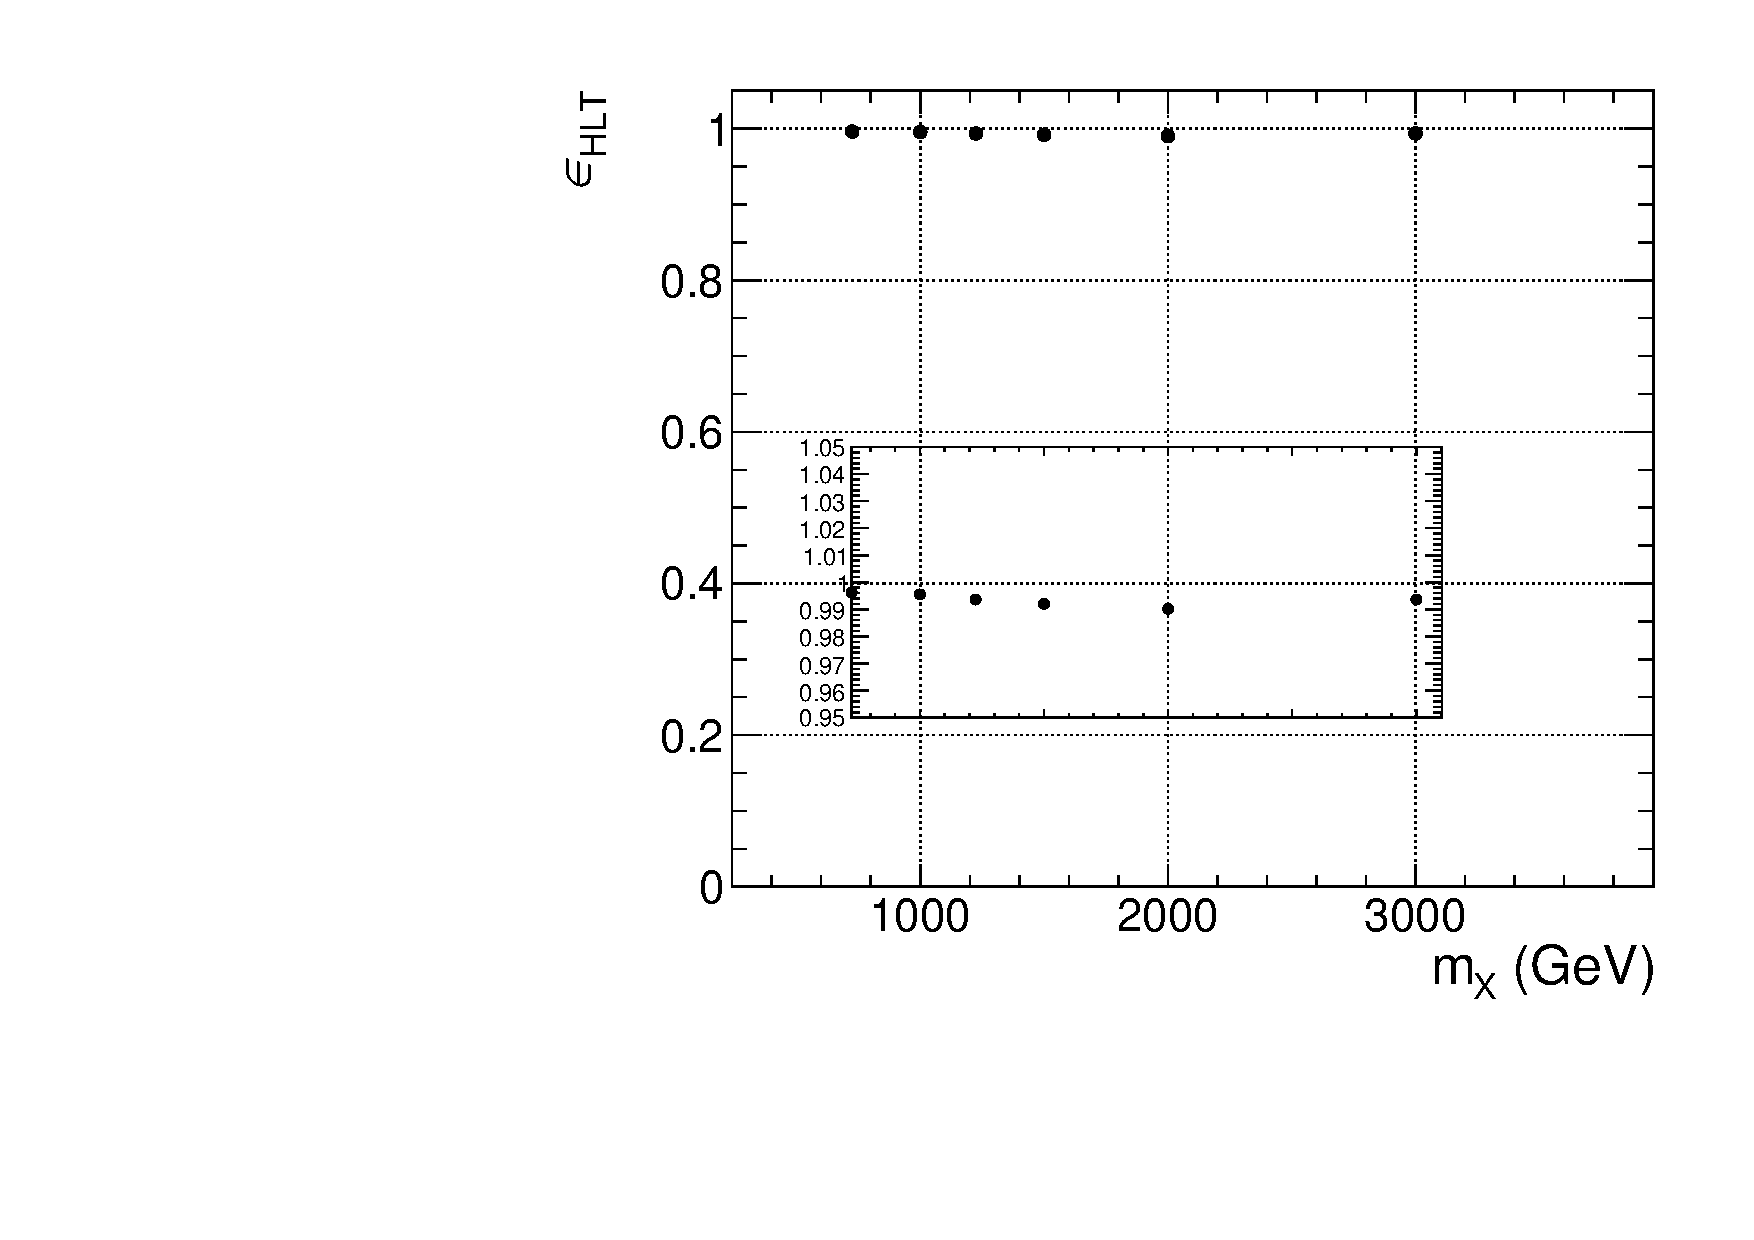
\includegraphics[angle=0,width=0.49\textwidth]{figures/eff_dipho60_EBEB_vs_mass}
	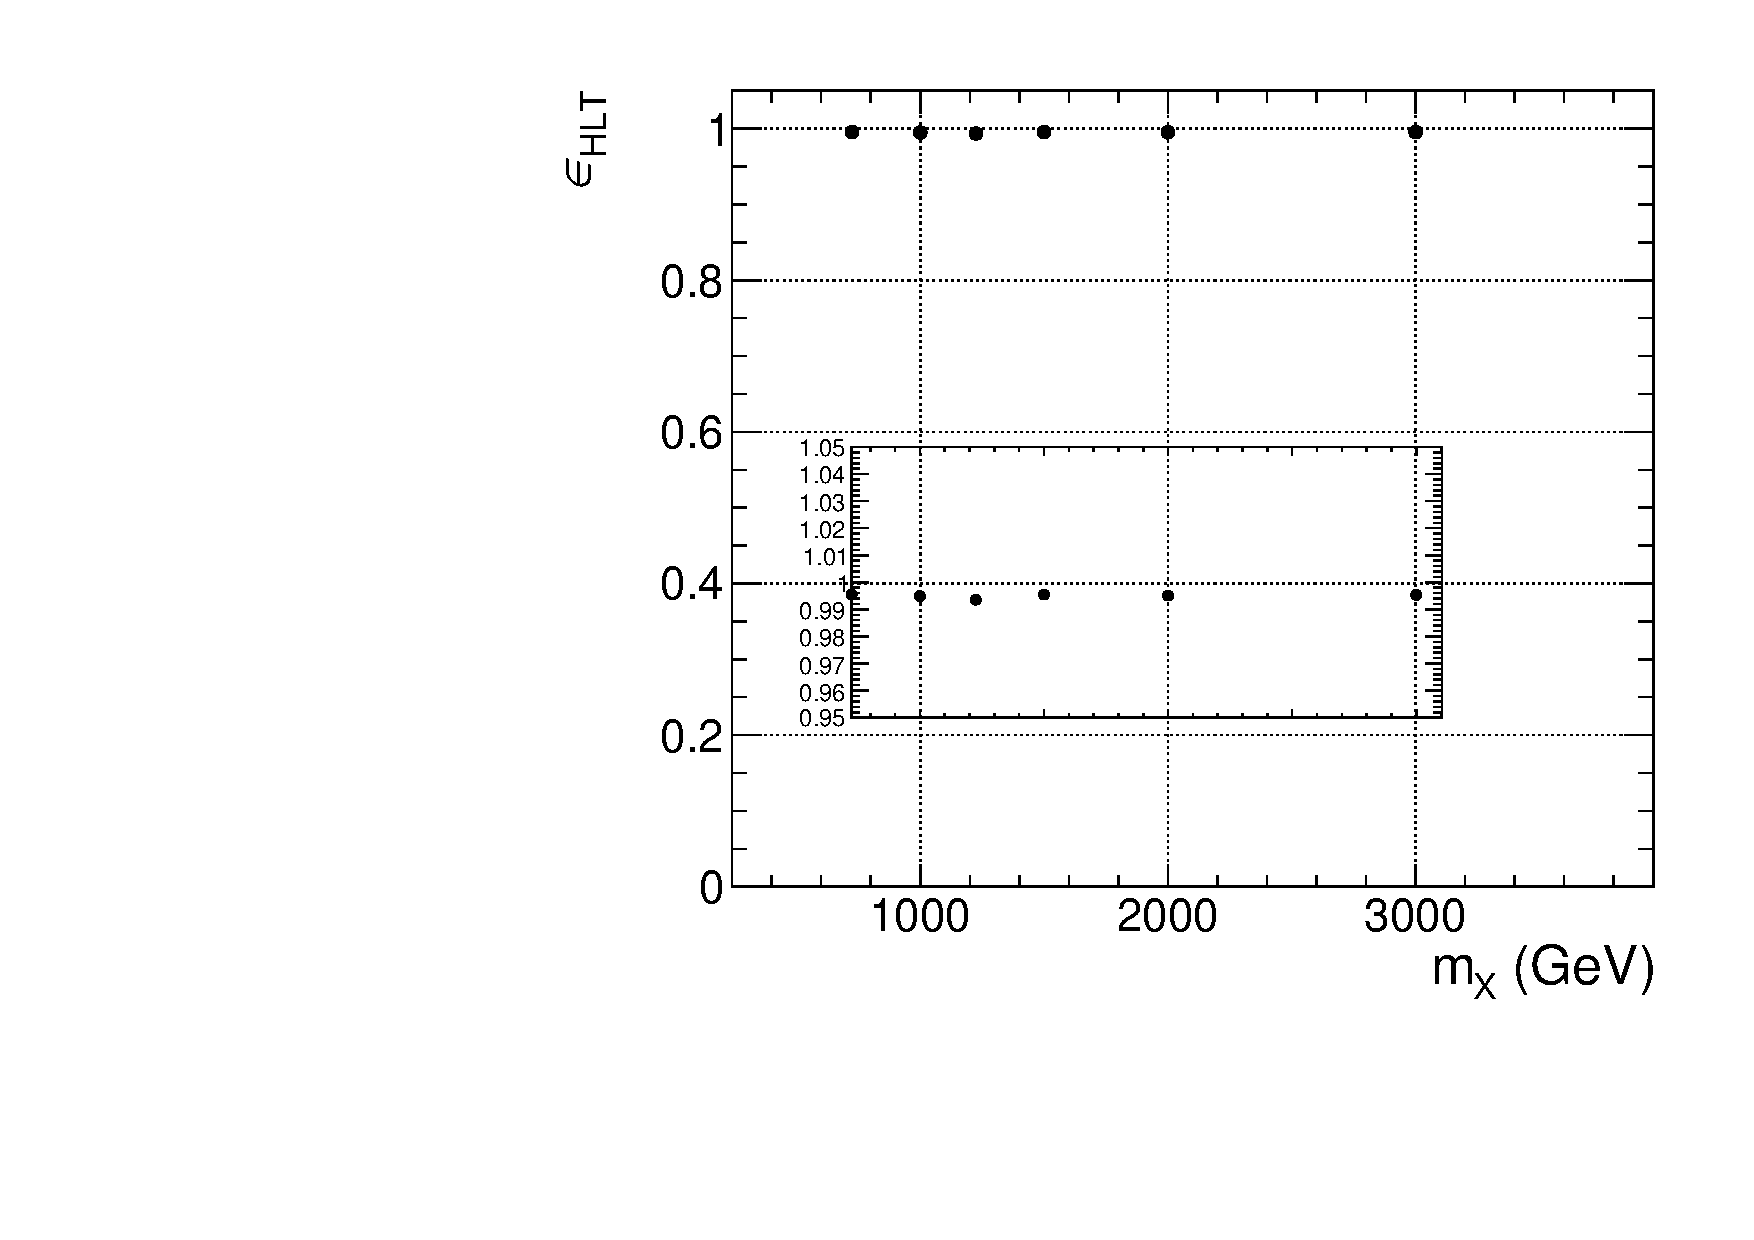
\includegraphics[angle=0,width=0.49\textwidth]{figures/eff_dipho60_EBEE_vs_mass}
	\caption{The absolute efficiency of the \texttt{HLT\_DoublePhoton60} trigger (measured using a simulated diphoton sample) as a function of $m_\mathrm{X} =\mgg$ in the EBEB (left) and EBEE (right) categories. The inner boxes show a zoomed-in region of the $y$-axis.}
	\label{fig:absolute_trigger_efficiency}
\end{figure}

To protect against potentially missing high-mass diphoton candidates at the trigger level, the backup trigger \texttt{HLT\_ECALHT800} is applied in addition to \texttt{HLT\_DoublePhoton60}. This triggers solely on the presence of large energy deposits in the ECAL without imposing additional criteria, such as a selection in \texttt{HLT\_DoublePhoton60} that could be responsible for causing the diphoton candidates to be rejected. The contribution from \texttt{HLT\_ECALHT800} to the analysis dataset is minimal (yielding $\sim$10 events).


\subsection{Event Preselection}

After trigger selection, candidate diphoton events are required to satisfy the following kinematic selection:
\begin{itemize}
	\item{each photon candidate is required to have $\pt>75\GeV$;}
	\item{one photon is required to be in the EB with $|\eta| < 1.4442$, and another in either the EB or in an EE, where it must have $1.566 < |\eta| < 2.5$;}
	\item{the photon pair must satisfy $\Delta R > 0.45$; and}
	\item{$\mgg>500\GeV$.}
\end{itemize}
\correction{The trigger efficiency measurements are one of the motivations for the photon $\pt>75\GeV$ and $\mgg>500\GeV$ requirements.} In this analysis, there are two signal regions considered: one with both photons in the EB, denoted EBEB, and the other with one photon in the EB and the other in either EE, denoted EBEE. Events with both photon candidates in the EEs are dominated by SM production and have negligible sensitivity to the target BSM signal, and thus are omitted from this analysis. Additional categories were considered, but were also excluded for this reason. We use the fiducial region of the ECAL, defined with a restricted $\eta$ range, as specified above, which rejects events outside of the tracker coverage and in the gap between the EB and EEs. The $\eta$ coordinate specifying this region corresponds to that of the supercluster position with respect to the fixed detector coordinate system, i.e., it is not relative to the shifting position of the primary vertex of each event. The $\Delta R$ requirement has a minimal effect on the overall event selection, but is motivated by a consistency requirement with the background simulation, as explained in Section~\ref{sec:real_background}. If more than one diphoton candidate satisfies this set of selection criteria, only the photon pair with the largest scalar sum of photon \pt is retained. 

The CMS standard primary vertex algorithm, as described in Section~\ref{sec:track_vertex}, is suboptimal when used for events based on neutral particles because these particles do not contribute to the selection variable $\sum{\pt^2}$ of charged particle tracks. In this case, improvements to the vertex finding can be made by analyzing the correlation between observables related to tracks recoiling against the diphoton system. The algorithm used by the $H \to \gamma\gamma$ analysis~\cite{Khachatryan:2014ira,Sirunyan:2018ouh} is incorporated in this analysis and is based on using this information as input to a multivariate classifier (a BDT). This algorithm is found to converge to the standard primary vertex algorithm at high \mgg. For diphoton events above $\mgg>500\GeV$, the interaction vertex is correctly assigned 90\% of the time, as measured in simulation and compared against data. If the position of the vertex along the $z$-axis is known to better than about 10~mm, then the diphoton mass resolution is dominated by the photon energy resolution. This is achieved by this algorithm at high \mgg.


\subsection{Photon Identification}

A dedicated set of photon identification criteria were developed for this analysis, tuned for high-mass photons. These criteria are based on photon shower shape and isolation variables, which help suppress misidentifications from jets and electrons (described further in Section~\ref{sec:fake_background}) while providing a high selection efficiency. One or two jets can fragment in such a way as to mimic a photon signature in the ECAL, causing the jet to be misreconstructed as a photon. For example, the decay of a neutral pion to two photons, $\pi^0 \to \gamma\gamma$, can fake a photon signature when both photon showers overlap in the ECAL. Electron showers are similar to photon showers in the ECAL, and if tracks are not properly assigned to an electron, they can fake a photon signature as well. In order to improve photon purity, we use identification criteria for photon candidates that are sensitive to the presence of more than one electromagnetic shower in the ECAL and to extra activity around the shower. Individual shower shape and isolation variables are used to achieve this.

The lateral shower shape variable \sieie is the spatial second moment of the supercluster about its average $\eta$ position. It can be thought of as the log energy-weighted RMS of the photon shower in units of the crystals, calculated as
\begin{equation}
	\sieie = \sqrt{
		\frac{\sum_{i \in 5{\times}5}(\eta_i-\bar{\eta})^2 w_i}{\sum_{i \in 5{\times}5} w_i}
	}
\end{equation}
with $w_i = \max{\left(0.0, 4.7 + \ln{E_i/E_{5{\times}5}}\right)}$, where $\bar{\eta}$ is the average supercluster position in $\eta$, $\eta_i$ is the $\eta$ coordinate of crystal $i$ in the $5{\times}5$ array, $E_i$ is the energy of crystal $i$, and $E_{5{\times}5}$ is the energy of the full $5{\times}5$ array centered on the seed crystal. A larger value of \sieie indicates a larger photon shower, essentially measuring the width of the photon shower in the $\eta$ direction. Prompt photons are well isolated in \sieie. In fact, \sieie is part of a covariance matrix describing the spatial extension of the photon shower in $(\eta,\phi)$ space:
\begin{singlespace}
%\vspace*{-\baselineskip}
	\begin{equation*}
		\begin{pmatrix}
			\sigma_{i\eta i\eta} & \sigma_{i\eta i\phi} \\
			\sigma_{i\eta i\phi} & \sigma_{i\phi i\phi} \\
		\end{pmatrix}
		\vspace*{\baselineskip}
	\end{equation*}
\end{singlespace}\noindent\ignorespaces
where \sipip and \sieip have analogous definitions as for \sieie. The variable \sipip is used in the background calculation, as described in Section~\ref{sec:fake_background}. High-energy photons causing saturation in the ECAL will have an effective wider shower in \sieie, as shown in Fig.~\ref{fig:sieie_sat}. The shower only appears wider since the central peak in the \sieie distribution is suppressed, due to the readout suppression above a certain threshold. In Fig.~\ref{fig:sieie_sat}, the tall edge on the left of the \sieie distributions are understood to be caused by prompt photons depositing their energy into the cracks between the ECAL crystals along the $\eta$ direction.

\begin{figure}[!htbp]
	\centering
	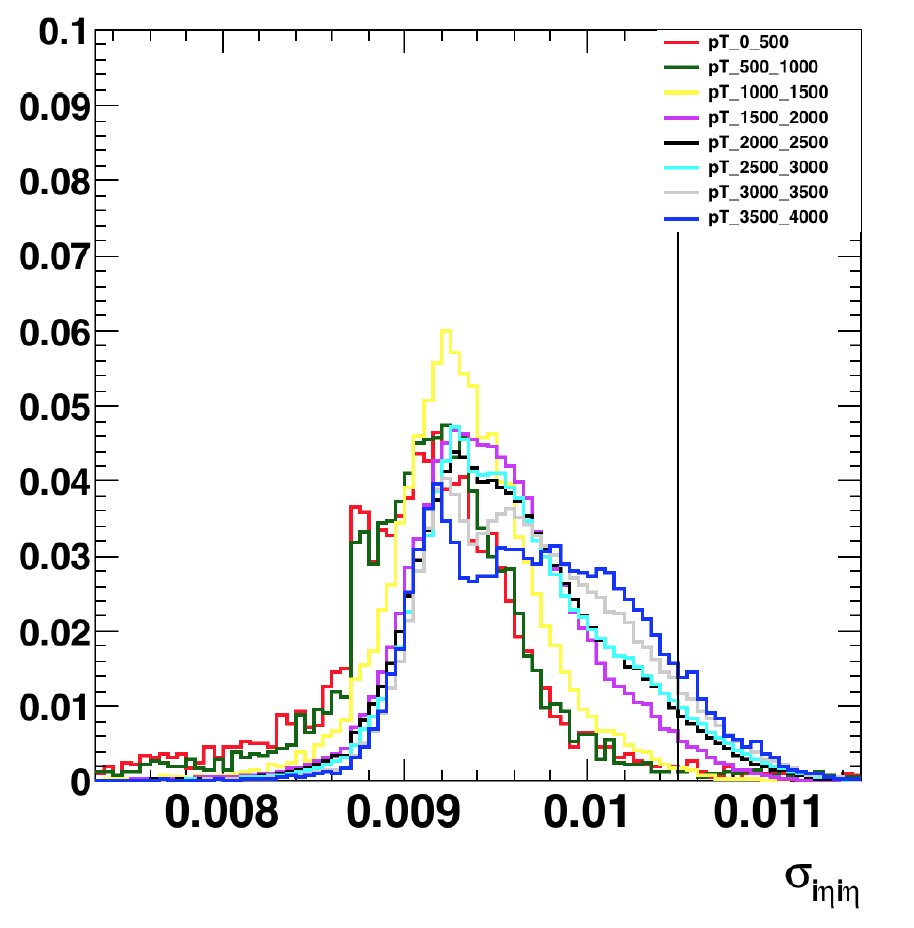
\includegraphics[width=0.49\textwidth]{figures/sieie_sat_old}
	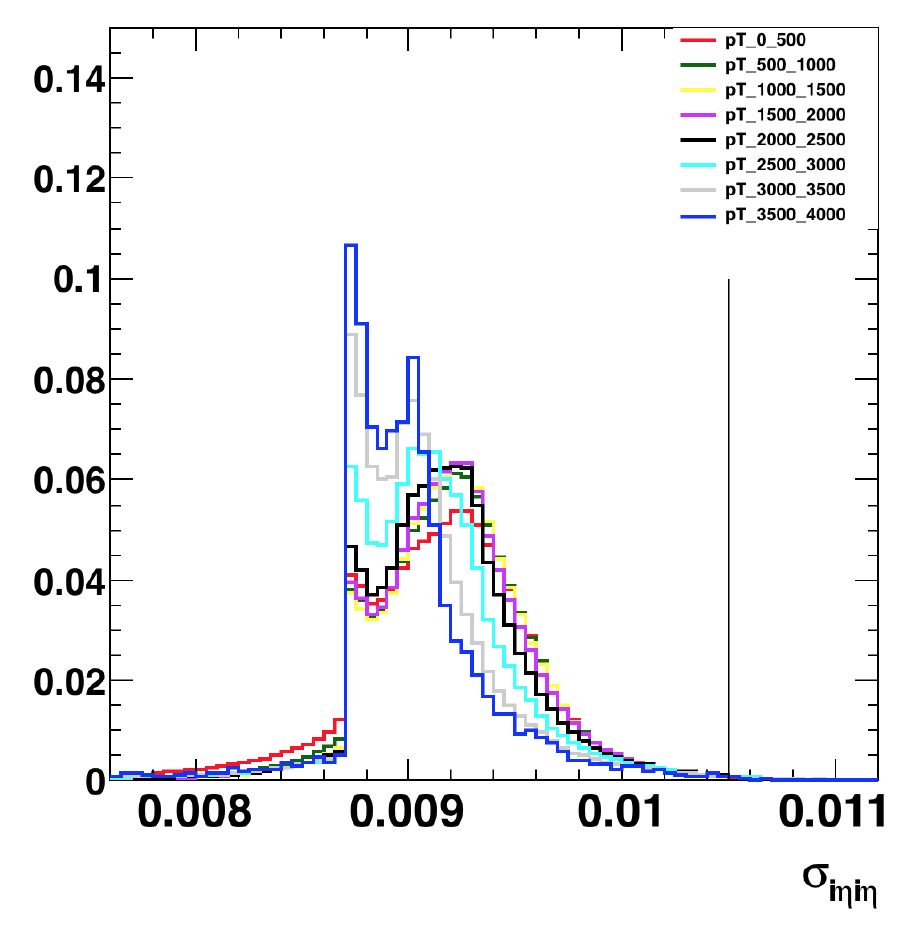
\includegraphics[width=0.49\textwidth]{figures/sieie_notSat_old}
	\caption{A plot of \sieie in various photon \pt bins for saturated (left) and unsaturated photons (right) in the EB. The vertical line is at the value of 0.0105.}
	\label{fig:sieie_sat}
\end{figure}

The variable \hoe, as defined above in Section~\ref{sec:trigger}, is the ratio of the hadronic to electromagnetic energy fraction of the photon candidate. This variable is close to zero for prompt photons, as the photon shower is well contained in the ECAL with little leakage into the HCAL. The \rnine variable is defined as the energy sum of the $3{\times}3$ array of crystals centered on the seed crystal divided by the energy of the supercluster. \rnine is sensitive to photon conversions, with unconverted photons having high values.

Isolation variables are based on the total scalar \pt sum of PF candidates assigned to the selected vertex with coordinates $(\eta,\,\phi)$ reconstructed within a cone of size $\DR = 0.3$ around the photon candidate with coordinates $(\eta_\gamma,\,\phi_\gamma)$, where $\DR = \sqrt{\smash[b]{(\eta - \eta_\gamma)^2 +(\phi-\phi_\gamma)^2}}$. In cases where the PF candidates share part of their energy with the photon candidate, they are excluded from the isolation sums. Separate variables are constructed for PF charged hadrons (\chiso) and PF photons (\phoiso). Prompt photons are well isolated for both variables. These PF candidates are calculated with respect to the diphoton vertex chosen using the $\mathrm{H} \to \gamma\gamma$ BDT. The \phoiso variable was found to be sensitive to both pileup and photon \pt. The corrected photon isolation has been pileup subtracted with \pt dependence removed according to:
\begin{equation}
	\corphoiso = \alpha + \phoiso - \rho A - \kappa \pt
\end{equation}
where $\kappa$ is a coefficient governing the \pt dependence; $\rho$ is the average pileup $\pt$ flow density per unit area in the event, calculated using the jet area method~\cite{Cacciari:2007fd,Cacciari:2008gn}; $A$ is an effective area, which is the geometrical area of the isolation cone times an $\eta$-dependent correction factor; and $\alpha$ is an empirical constant chosen to make the corrected isolation peak near zero. General pileup removal algorithms utilized by the CMS Collaboration are found in Ref.~\cite{CMS-PAS-JME-14-001}. The values for $\alpha$, $A$, and $\kappa$ are listed in Table~\ref{tab:corphoiso_values} based on the $\eta$ coordinate of the supercluster (\scEta). When \corphoiso is considered in simulated data, an additional stochastic correction is applied to account for the mismodeling of the pileup dependence of \phoiso in simulation. This correction assumes that the effect of pileup on \phoiso is to add a discrete number of photons in its isolation cone.

\begin{table}[!htbp]
	\centering
	\caption{Parameters used in the definition of \corphoiso based on the $\eta$ coordinate of the supercluster (\scEta).}
	\vspace{\baselineskip}
	\begin{tabular}{l|ccc}
	\hline \hline
	Detector region       & $\alpha$ ({\GeVns}) & $A$ & $\kappa$ \\
	\hline
	$|\scEta|<0.9$        & 0.99 & 0.15  & 0.0016 \\
	$0.9<|\scEta|<1.4442$ & 0.99 & 0.13  & 0.0016 \\
	$1.566<|\scEta|<2.0$  & 0.77 & 0.093 & 0.00075  \\
	$2.0<|\scEta|<2.2$    & 0.77 & 0.15  & 0.00075  \\
	$2.2<|\scEta|<2.5$    & 0.77 & 0.21  & 0.00075  \\
	\hline \hline
	\end{tabular}
	\label{tab:corphoiso_values}
\end{table}

Electrons and photons leave similar energy deposits in the ECAL, so an electron veto is applied to reject electrons in the selection. Electrons are vetoed based on hits in the silicon pixel and strip trackers with a further check to ensure photon candidates associated with electron tracks are incompatible with those resulting from photon conversions. This is known as the conversion-safe electron veto (CSEV).

The cut values applied to each of these identification variables are listed in Table~\ref{tab:photon_ID}, separately for photons in the EB and EEs. This collection of photon identification criteria is known as the high-\pt photon ID. \correction{This ID was developed and tuned specifically for this analysis, with significant contributions from the author of this dissertation.}


\begin{table}[!htbp]
	\caption{The high-\pt photon ID. The cut values are listed for the different identification variables. For \sieie, the values in parenthesis correspond to saturated photons in the ECAL.}
	\centering
	\vspace{\baselineskip}
	\begin{tabular}{c|cccccc}
		\hline \hline
		\vspace*{-4.5mm} & & & & & \\
		\vspace*{+0.1mm}Photon category & \chiso ({\GeVns}) & \corphoiso ({\GeVns}) & \hoe & \sieie & \rnine & CSEV \\
		\hline
		EB & 5 & 2.75 & 0.05 & 0.0105 (0.0112) & 0.8 & applied \\
		EE & 5 & 2.0  & 0.05 & 0.028 (0.030) & 0.8 & applied \\ 
		\hline \hline
	\end{tabular}
	\label{tab:photon_ID}
\end{table}

The background which remains from misidentifications not suppressed by the high-\pt photon ID is discussed in Section~\ref{sec:fake_background}.


\subsection{Selection Efficiency}

The efficiency of the high-\pt photon ID was measured using the tag-and-probe technique, similar to the procedure done in Ref.~\cite{CMS:2011aa}. This technique is used in both data, using a sample of electron-triggered events, and in simulation, using a $Z \to e^+ e^-$ sample. The tag is an electron required to be in the event, with $\pt > 30\GeV$, passing the standard CMS electron ID. The probe is a photon with $\pt > 20\GeV$ passing the high-\pt photon ID with an inverted CSEV. The invariant mass of the tag-and-probe system is required to be between 70-110\GeV. Figure~\ref{fig:tnp_eff} shows the photon selection in the EB and EE regions, including data-over-simulation scale factors. The overall efficiency is about 90 (87)\% for single photons in the EB (EE) region. The scale factors are compatible with unity, but are still applied to the simulation described in Chapters~\ref{ch:background}~and~\ref{ch:signal}.

\begin{figure}[!htbp]
	\centering
  	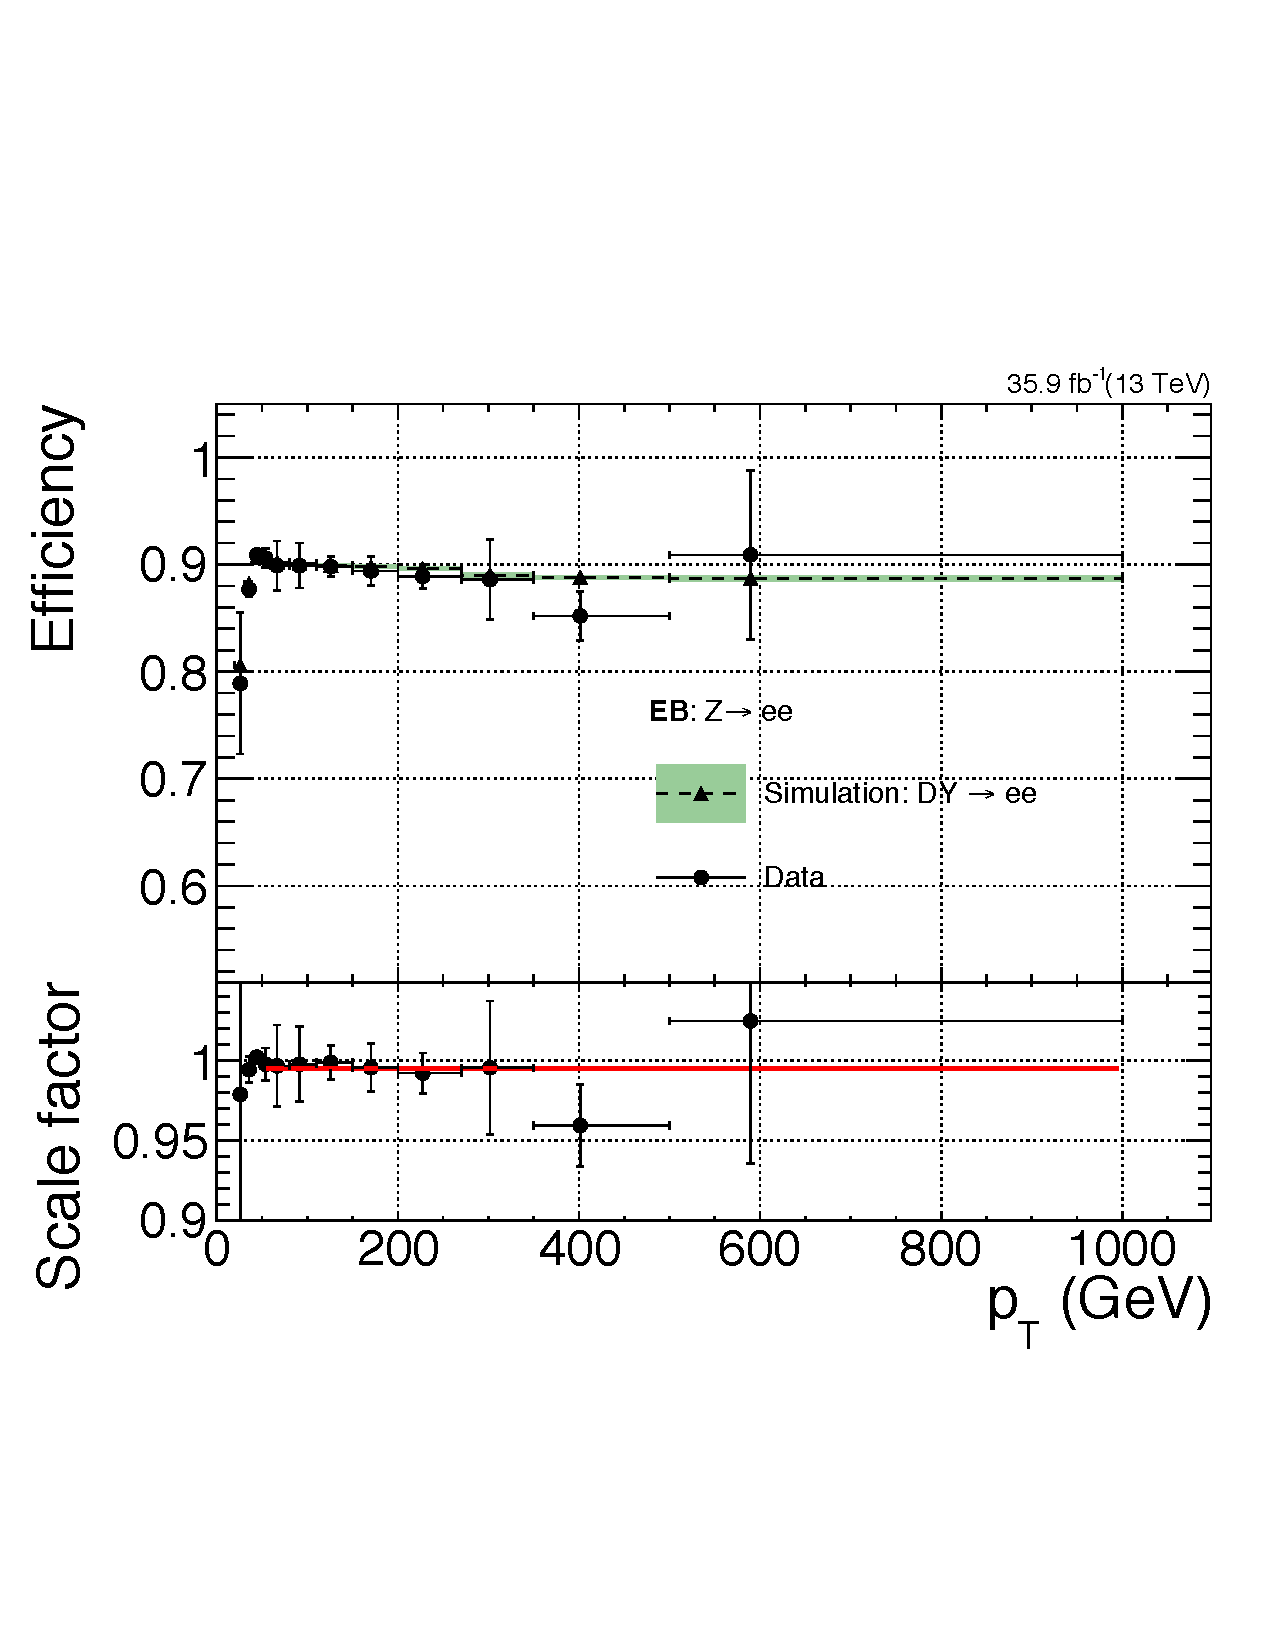
\includegraphics[angle=0,width=0.49\textwidth]{figures/sf_vs_pt_EB2.pdf}
	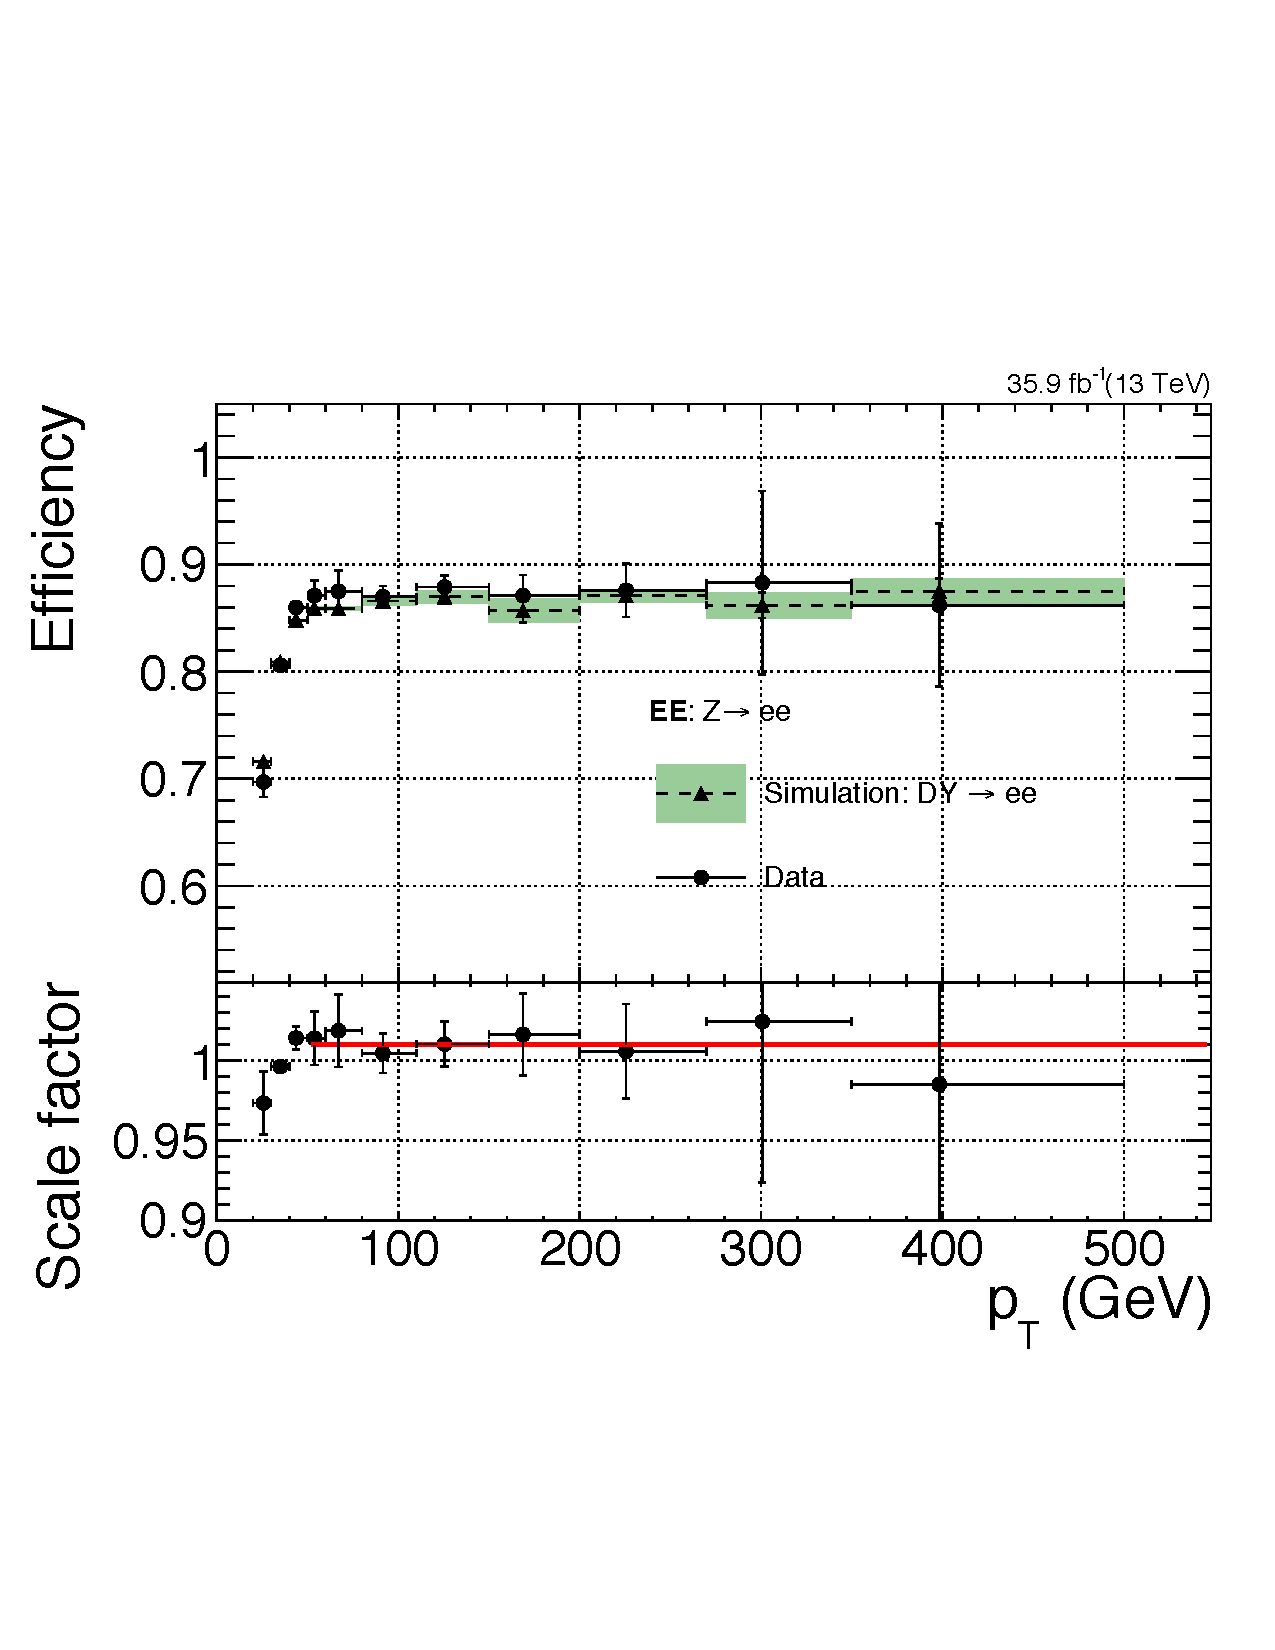
\includegraphics[angle=0,width=0.49\textwidth]{figures/sf_vs_pt_EE2.pdf}
	\caption{Photon selection efficiency (top) in the EB (left) and EE (right) regions and the associated data-over-simulation scale factors (bottom). The statistical and systematic errors are shown.}
	\label{fig:tnp_eff}
\end{figure}

The result of considering the event selection efficiency ($\varepsilon$) and detector acceptance ($A$) together is shown in Fig.~\ref{fig:eff_x_acc}. This was measured using simulation, similar to the samples described in Chapter~\ref{ch:signal}, using events of known \mgg and determining which accepted events pass the high-\pt ID requirements. The combination of each across both analysis categories is approximately 60\%.

\begin{figure}[!htb]
    \centering
    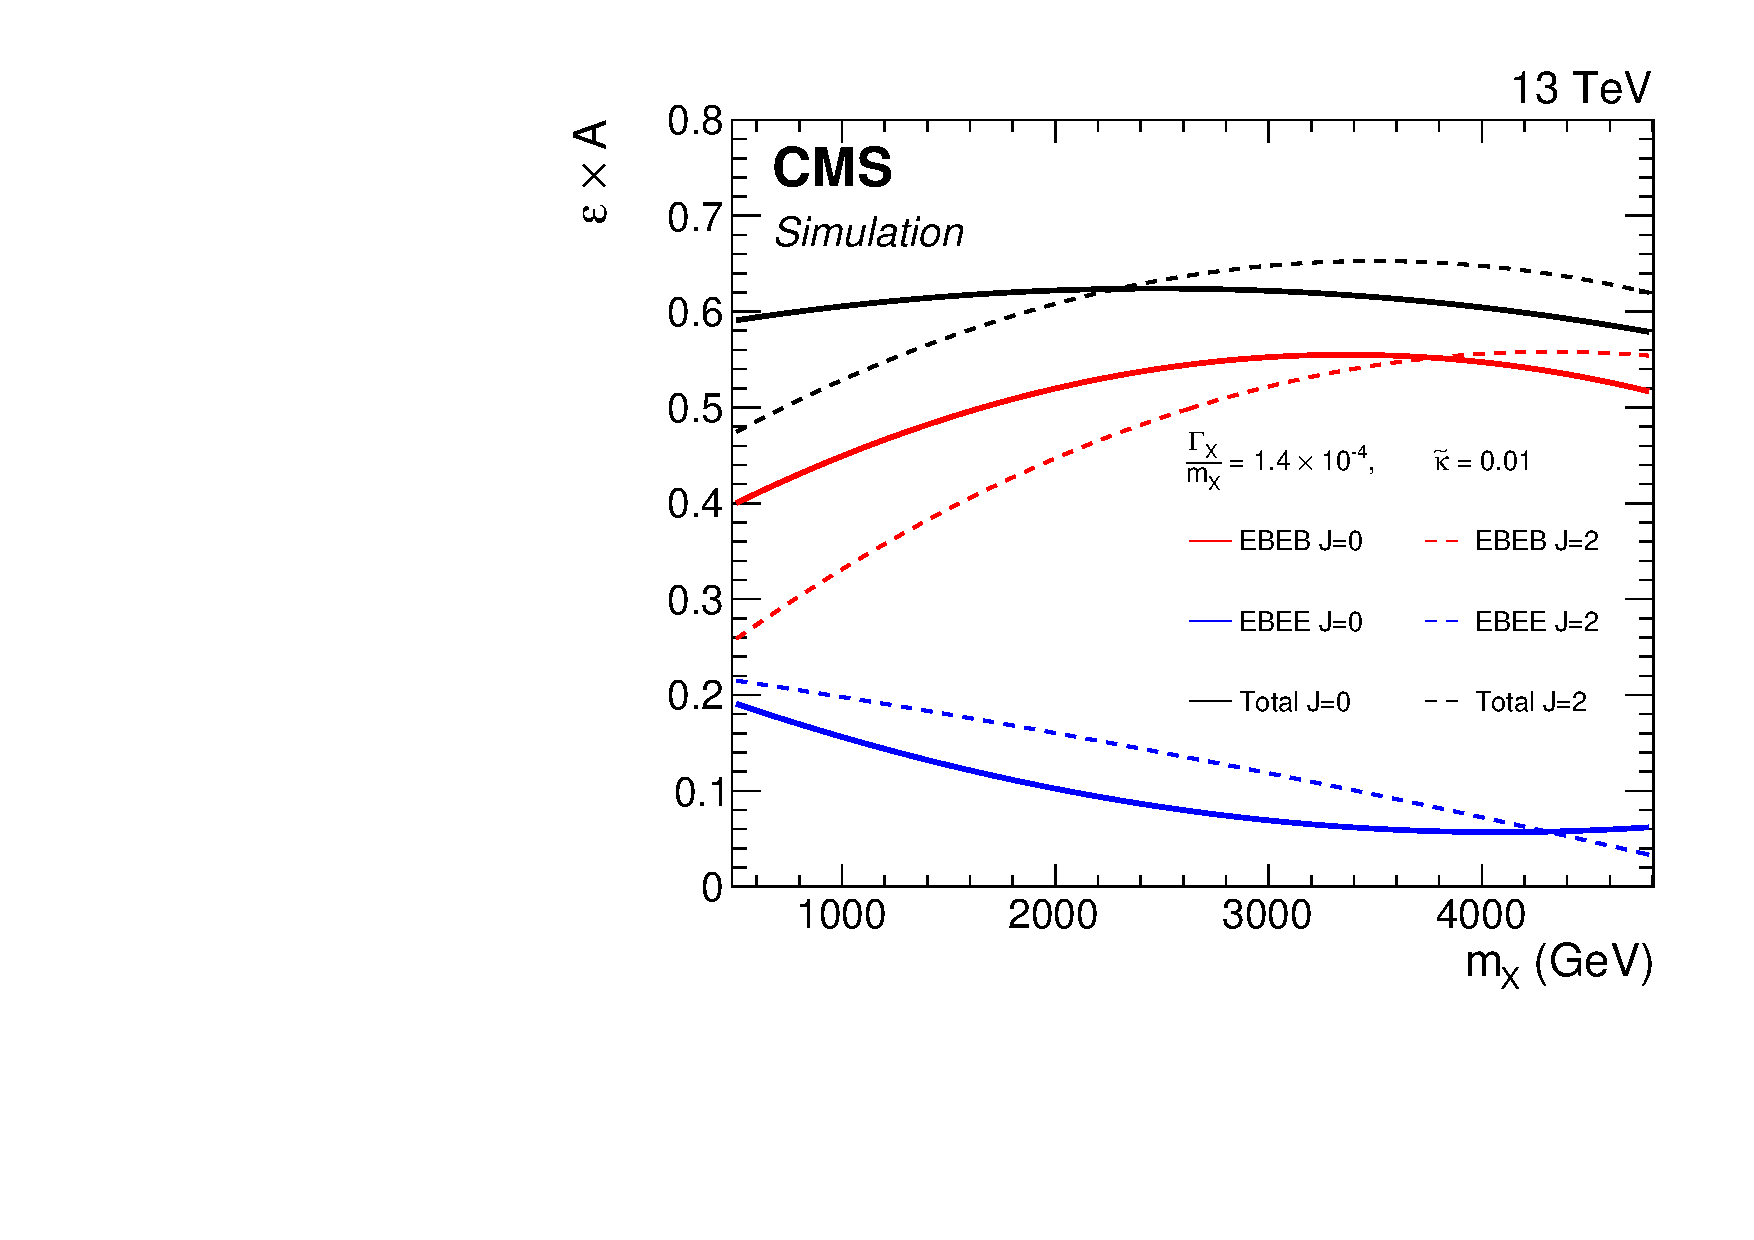
\includegraphics[width=0.65\textwidth]{figures/eff_x_acc_k001.pdf}
    \caption{The product of the event selection efficiency ($\varepsilon$) and the detector acceptance (A) is shown as a function of signal resonance mass $m_{\mathrm{X}} = \mgg$ for the $\Gamma_{\mathrm{X}}/m_{\mathrm{X}}=1.4\times10^{-4}$ signal width hypothesis. The total (black), EBEB (red), and EBEE (blue) curves are shown for the spin (J) hypotheses $\mathrm{J}=0$ (solid line) and $\mathrm{J}=2$ (dashed line).
    }
    \label{fig:eff_x_acc}
\end{figure}


\subsection{Datasets}

The datasets used in this analysis were recorded in 2016 and correspond to an integrated luminosity of 35.9\fbinv. They were produced using LHC proton-proton collisions at $\sqrt{s} = 13\TeV$ and recorded by the CMS detector. Each dataset is listed in Table~\ref{tab:data_samples} according to their internal CMS path and corresponding integrated luminosity. These \texttt{DoubleEG} triggered primary datasets contain at least two electron or photon candidates.

\begin{table}[!htbp]
	\caption{The analysis datasets, each listed with their CMS path name and corresponding integrated luminosity.}
	\centering
	\vspace{\baselineskip}
	\begin{tabular}{lc}
	\hline \hline
	Dataset path & Int. lumi.  (\fbinv) \\
	\hline
	/DoubleEG/Run2016B-03Feb2017\_ver2-v2          &  5.788 \\
	/DoubleEG/Run2016C-03Feb2017-v1/MINIAOD        &  2.573 \\
	/DoubleEG/Run2016D-03Feb2017-v1/MINIAOD        &  4.248 \\
	/DoubleEG/Run2016E-03Feb2017-v1/MINIAOD        &  4.009 \\
	/DoubleEG/Run2016F-03Feb2017-v1/MINIAOD        &  3.102 \\
	/DoubleEG/Run2016G-03Feb2017-v1/MINIAOD        &  7.540 \\
	/DoubleEG/Run2016H-03Feb2017\_ver2-v1/MINIAOD  &  8.391 \\
	/DoubleEG/Run2016H-03Feb2017\_ver3-v1/MINIAOD  &  0.215 \\
	\hline \hline
	\end{tabular}
	\label{tab:data_samples}
\end{table}


